\onecolumn
{
    \hypersetup{linkcolor=black}
    \parskip=0em
    \renewcommand{\contentsname}{Contents}
    \tableofcontents
    \addtocontents{toc}{\protect\setcounter{tocdepth}{3}}
}

\newpage

\section{Appendix}
\subsection{LLM usage}
The large language model (LLM) was utilized as a writing assistant during the preparation of this manuscript. Its application was strictly limited to improving the clarity and grammatical accuracy of the text. Specific uses included rephrasing sentences for better flow and translating initial concepts and drafts from Chinese to English. All core scientific contributions, including the conceptualization of our \method framework, the design of the methodology and experiments, and the analysis and interpretation of the results, are solely the work of the authors. The authors take full responsibility for all claims and the final content of this paper.

\subsection{Experimental Setup}
\label{experiment_details}
\subsubsection{Datasets}

Here, we provide a detailed introduction to the datasets used in this paper:

\begin{itemize}[left=0pt]
    \item \textbf{GAIA}~\citep{mialon2023gaiabenchmarkgeneralai} serves as a benchmark designed to evaluate next-generation LLMs that possess enhanced capabilities through the incorporation of tools, efficient prompting strategies, and access to external search resources. This benchmark comprises over 450 challenging questions, each with a clear and unequivocal answer, necessitating varying degrees of tooling and autonomy for resolution. Accordingly, the questions are categorized into three distinct levels: Level 1 is expected to be solvable by proficient LLMs, while Level 3 signifies a substantial increase in the model's capabilities. Each level includes a fully public development set for validation purposes, as well as a test set containing private answers and associated metadata. In our experiments, we utilize the test set, which encompasses 164 tasks.
    \item \textbf{GSM-hard}~\citep{gao2022pal} is an advanced version of the GSM8K mathematics reasoning dataset~\citep{cobbe2021gsm8k}. This enhanced dataset presents models with increased challenges, featuring larger numerical values and more complex relationships within the problems.
    \item \textbf{AIME-2024}~\citep{HuggingFaceH4_AIME_2024} is a dataset comprising problems derived from the American Invitational Mathematics Examination (AIME) 2024. AIME is a prestigious mathematics competition for high school students, recognized for its challenging problems that span various mathematical domains. This benchmark serves multiple purposes: it evaluates the mathematical reasoning capabilities of LLMs, assesses their problem-solving abilities on complex mathematical challenges, and investigates AI performance on structured mathematical tasks.
    \item \textbf{HumanEval}~\citep{chen2021evaluatinglargelanguagemodels} is a dataset released by OpenAI that includes 164 programming problems, each containing a function signature, a docstring, a body, and several associated unit tests. These problems were handwritten to ensure that they were not included in the training dataset for code-generation models. This benchmark is crucial for evaluating code-generation models, providing a structured set of challenges in Python that facilitates the assessment of both the quality and correctness of code produced by language models.
    \item \textbf{MBPP}(Mostly Basic Python Problems Dataset)~\citep{austin2021programsynthesislargelanguage} comprises approximately 1,000 crowd-sourced Python programming problems that are specifically designed to be solvable by entry-level programmers. The dataset covers essential programming fundamentals and standard library functionalities. Each problem includes a task description, a corresponding code solution, and three automated test cases.
    \item \textbf{DROP}(Data Retrieval Open Answering)~\cite{dua-etal-2019-drop} is a reading comprehension benchmark that requires discrete reasoning over paragraphs. This dataset consists of 96,000 questions developed through crowd sourcing and adversarial methods. It challenges systems to resolve references within the questions, which may point to multiple input positions. The tasks entail performing discrete operations, such as addition, counting, and sorting, necessitating a substantially more comprehensive understanding of paragraph content than that demanded by prior datasets. In our experiment, we sampled 800 tasks for evaluation.
\end{itemize}


\subsubsection{Baselines}
\label{appendix:baselines}
\begin{itemize}[left=0pt]
    \item \textbf{Vanilla} is the original Large Language Model (LLM) that processes input using only the question and a basic prompt, without any prompt engineering or external tool integration. This straightforward approach emphasizes the model's inherent capabilities in handling natural language tasks. By operating in this simplistic manner, Vanilla LLM serves as a critical baseline for evaluating the performance of more advanced techniques that incorporate sophisticated prompt strategies or additional tools, thereby providing valuable insights into the effectiveness of various methodologies in natural language processing.
    \item \textbf{CoT-SC}(Chain-of-Thought Self-Consistency)~\citep{wang2023selfconsistencyimproveschainthought} serves as a baseline for enhancing the reasoning capabilities of language models. This approach generates multiple reasoning chains, which are then aggregated to produce a coherent summary. By leveraging self-consistency, CoT-SC improves the reliability of the model's outputs, allowing for better performance in complex reasoning tasks. This structured process facilitates deeper analysis of the model's thought processes, providing a foundation for comparing more advanced reasoning strategies and understanding their impact on overall performance.
    \item \textbf{MetaAgent}~\citep{zhang2025metaagentautomaticallyconstructingmultiagent} is a groundbreaking framework designed to automatically construct multi-agent systems by specifying the objectives of a given task. A distinctive feature of MetaAgent is its ability to generate these multi-agent systems without relying on external training data. This capability allows the produced multi-agent systems to effectively address all scenarios within the specified task domain. The underlying architecture of the Multi-Agent System is based on Finite State Machines(FSM), which facilitates structured decision-making and state transitions, thereby enhancing the system's operational efficiency and adaptability.
    \item \textbf{OWL}(Open Web Language)~\citep{hu2025owl} serves as a foundational framework for knowledge representation in multi-agent systems. By enabling agents to process and reason over complex data in a machine-readable format, OWL is crucial for facilitating interoperability among diverse agents. It allows for the creation of ontologies that define intricate relationships and constraints within the environment, thereby enhancing collaborative behaviors among agents. The expressive power of OWL supports advanced inference capabilities, empowering agents to share knowledge effectively and make informed decisions. This framework establishes a robust baseline for evaluating and enhancing the performance of multi-agent systems in various applications.
    \item \textbf{Smolagent}~\citep{smolagents} is a lightweight library designed to facilitate the development and implementation of AI agents that can think and operate using code. It emphasizes simplicity and efficiency, enabling users to create multi-agent systems with minimal code. Smolagent's architecture allows for smart threading, dependency management, and context sharing, making it ideal for orchestrating complex tasks. By providing a streamlined framework, Smolagent serves as a foundational model for evaluating the performance and capabilities of more advanced agent-based systems in various applications.
    \item \textbf{OAgents}~\citep{zhu2025oagentsempiricalstudybuilding} is a modular multi-agent framework that conducts a thorough empirical study of key agent components (planning, memory, tool use, test-time scaling) on benchmarks such as GAIA and BrowseComp. It delivers great performance among open-source agent frameworks. Importantly, OAgents builds on the lightweight agentience model provided by Smolagent (which emphasises code-based agent orchestration and minimal overhead) and extends it with fine-grained task decomposition, dynamic workflow adaptation, multi-source web browsing and more extensive tool and memory modules.
    \item \textbf{AWorld}~\citep{yu2025aworldorchestratingtrainingrecipe} is an open-source framework for large-scale agent–environment interaction, designed to operationalize the “learning from practice” paradigm in agentic AI. It features a hierarchical multi-agent architecture composed of specialized agents such as the \emph{Execution Agent}, which performs primary reasoning and tool-use operations, and the \emph{Guard Agent}, which intervenes at critical steps to verify and refine intermediate outcomes. AWorld adopts a modular design supporting dynamic supervision, context tracking, and distributed orchestration, enabling efficient coordination across diverse tasks and environments. By treating agents and tools as interchangeable components within a unified orchestration layer, it facilitates flexible composition, concurrent execution, and fine-grained control over reasoning workflows, illustrating a scalable and extensible paradigm for constructing adaptive multi-agent systems.
\end{itemize}



\subsection{Implementation details}
\label{implementation_details}

\begin{table*}[t]
    \centering
    \caption{Hyperparameter settings for the Heuristic-Based Adaptive Filter across different benchmarks. The symbols correspond to the definitions in Algorithm \ref{alg:adaptive_filter}.}
    \label{tab:hyperparams}
    \vspace{2mm} %
    \resizebox{\textwidth}{!}{%
    \begin{tabular}{llcccccc}
    \toprule
    \textbf{Condition} & \textbf{Parameter (Symbol)} & \textbf{GAIA} & \textbf{HumanEval} & \textbf{MBPP} & \textbf{AIME} & \textbf{DROP} & \textbf{GSM-Hard} \\
    \midrule
    \multirow{2}{*}{\textit{Inefficient}} 
        & Step Check Interval ($\tau_{\text{step}}$) & 8 & 6 & 4 & 4 & 4 & 4 \\
        & Loop Detection Window ($\tau_{\text{loop}}$) & 5 & 5 & 3 & 3 & 3 & 3 \\
    \midrule
    \textit{Excessive} 
        & Length Threshold ($\tau_{\text{len}}$) & \multicolumn{6}{c}{3000} \\
    \bottomrule
    \end{tabular}
    }
\end{table*}

In this section, we provide a detailed description of how the conceptual framework of \method{} is implemented in our codebase. Our implementation is centered around the \texttt{supervise\_and\_correct} function, which serves as the primary entry point for all supervisory actions. We structure our explanation following the same \emph{What, When, and How} logic presented in our main methodology.

\subsubsection{What to Supervise: The ActionStep Object}
Our supervision targets the discrete interaction steps performed by each agent within the MAS. In our framework, every such interaction is encapsulated in a data structure we refer to as an \texttt{ActionStep} object. This object contains all relevant information for a single step, including the agent's thought process (\texttt{model\_output}), the executed \texttt{tool\_calls}, the resulting \texttt{observations}, and an \texttt{error} attribute which is populated if an exception occurs. Our \method{} is implemented as a callback function that intercepts every \texttt{ActionStep} object generated by any agent in the system.

\subsubsection{When to Supervise: The Prioritized Adaptive Filter}
To avoid the prohibitive cost of constant intervention, we employ a lightweight, LLM-free adaptive filter. This filter is implemented as a prioritized conditional chain at the beginning of the \texttt{supervise\_and\_correct} function. It evaluates each \texttt{ActionStep} to determine if supervision is warranted. The conditions are checked in the following order of precedence:

\begin{enumerate}[nosep, leftmargin=15pt]
    \item \textbf{Sub-Agent Completion}: The highest priority is to check if the observation contains a final report from a sub-agent (identified by the presence of a \texttt{"\textless summary\_of\_work\textgreater"} string). If so, it triggers the specialized \texttt{Adaptive Observation Purification} strategy to distill the findings for the manager agent.
    \item \textbf{Error Occurrence}: If the \texttt{step.error} attribute is not \texttt{None}, the \texttt{Proactive Error Correction} strategy is triggered. Our implementation includes a defensive check to ensure this does not fire for known, non-critical tool failures that the base agent can handle.
    \item \textbf{Inefficient Behavior}: If no error is present, we then check for inefficiency using our heuristic-based \texttt{\_check\_for\_inefficiency} function. This function detects patterns such as hard loops (identical actions and observations) and excessive step counts for a given sub-task, triggering the \texttt{Guidance for Inefficiency} strategy.
    \item \textbf{Excessive Observation Length}: Finally, if none of the above conditions are met, the filter checks if the length of the \texttt{step.observations} string exceeds a pre-defined threshold $\tau_{\text{len}}$ (3,000 characters in our implementation). If it does, the general type of \texttt{Adaptive Observation Purification} strategy is activated.
\end{enumerate}

If none of these trigger conditions are met, the step is approved by default, thereby avoiding any unnecessary LLM-based supervision overhead. 
The filter’s sensitivity is governed by three key hyperparameters: $\tau_{\text{step}}$ and $\tau_{\text{loop}}$ modulate the detection of inefficient behaviors, while $\tau_{\text{len}}$ defines the threshold for identifying excessive observations.
The complete logic of this heuristic-based mechanism is formalized in Algorithm \ref{alg:adaptive_filter}.



\begin{algorithm}[t]
\caption{Heuristic-Based Adaptive Filter Logic}
\label{alg:adaptive_filter}
\begin{algorithmic}[1]
\Input Current execution history $\mathcal{H}$ (sequence of steps), Current observation $o$, Error status $e$
\Require Hyperparameters: $\tau_{\text{step}}$ (step check interval), $\tau_{\text{loop}}$ (loop detection window), $\tau_{\text{len}}$ (length threshold)
\Ensure Boolean flag $trigger$, Intervention context $c$

\State $trigger \gets \text{False}$
\State $c \gets \text{None}$

\Statex \Comment{\textit{Priority 1: Check for explicit runtime errors}}
\If{$e$ is \textbf{True}}
    \State \Return $(\text{True}, c_{\text{error}})$
\EndIf

\Statex \Comment{\textit{Priority 2: Check for inefficient behaviors}}
\State $N \gets \text{Length}(\mathcal{H})$
\If{$N > 0$ \textbf{and} $N \pmod{\tau_{\text{step}}} = 0$} \Comment{Periodic strategy check}
    \State \Return $(\text{True}, c_{\text{inefficient}})$
\EndIf

\If{$N \geq \tau_{\text{loop}}$} \Comment{Repetitive loop detection}
    \State $\mathcal{A}_{\text{recent}} \gets \text{GetLastToolCalls}(\mathcal{H}, \text{window}=\tau_{\text{loop}})$
    \If{$|\text{Unique}(\mathcal{A}_{\text{recent}})| = 1$}
        \State \Return $(\text{True}, c_{\text{inefficient}})$
    \EndIf
\EndIf

\Statex \Comment{\textit{Priority 3: Check for excessive information}}
\If{$\text{Length}(o) > \tau_{\text{len}}$}
    \State \Return $(\text{True}, c_{\text{excessive}})$
\EndIf

\State \Return $($trigger, $c)$
\end{algorithmic}
\end{algorithm}

\begin{figure}[!t] %
    \centering
    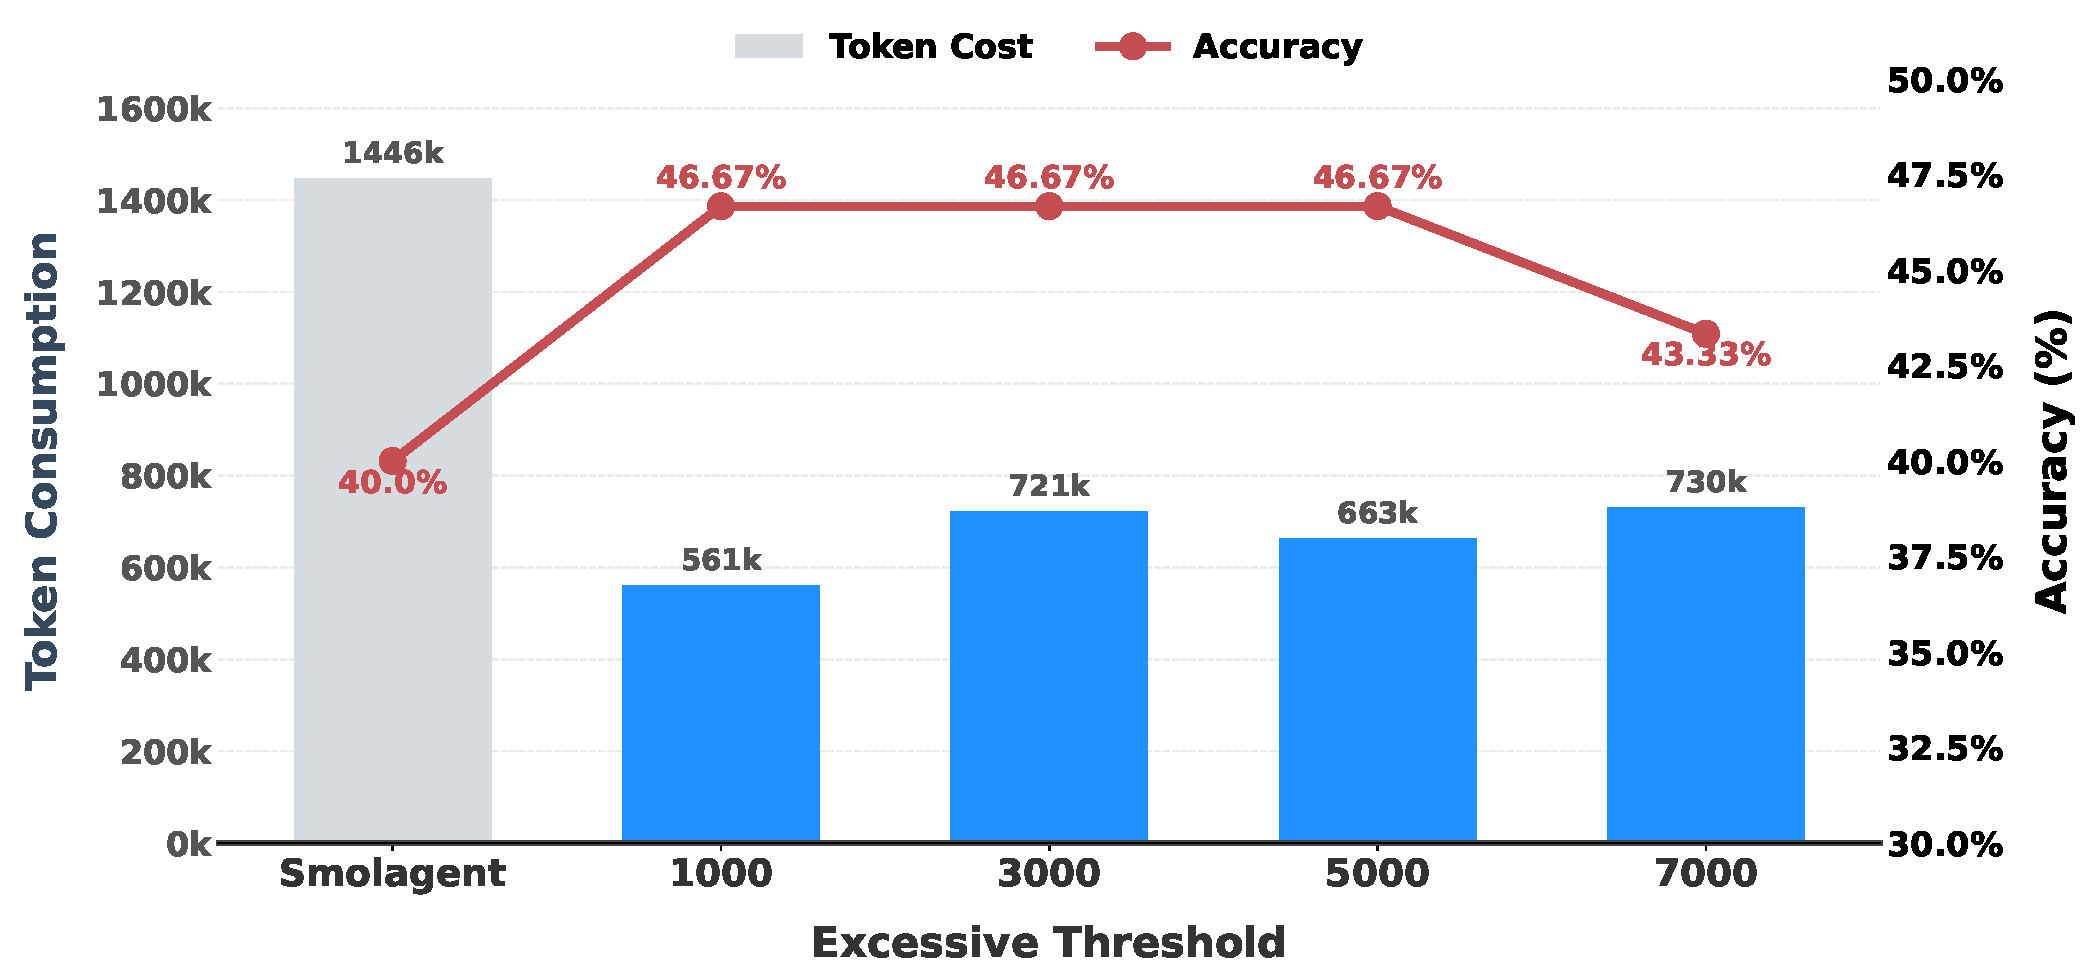
\includegraphics[width=0.9\linewidth]{resources/figures/excessive_thre_sensitivity.pdf}
    \caption{
        \textbf{Sensitivity analysis on excessive threshold ($\tau_{\text{len}}$).} Evaluated on GAIA subset (top-10 most token-intensive tasks per level).
    }
    \label{fig:sensitivity}
\end{figure}





\paragraph{Sensitivity analysis and hyperparameter configuration.}
Table \ref{tab:hyperparams} details the hyperparameter settings for our Heuristic-Based Adaptive Filter across different benchmarks. We conducted a sensitivity analysis on the excessive observation length threshold ($\tau_{\text{len}}$) using the representative subset of the GAIA benchmark (top-10 most token-intensive tasks per level), as illustrated in Figure \ref{fig:sensitivity}. The results indicate that our method maintains robust performance across a wide range of threshold values, demonstrating its adaptability without significant degradation. Although slight performance peaks are observed at $\tau_{\text{len}}=1000$ and $\tau_{\text{len}}=5000$, we selected $3000$ as the default value. This choice strikes a prudent balance between sensitivity (catching enough noise) and specificity (preserving useful context), ensuring optimal performance across diverse tasks while minimizing the risk of over-intervention.

\paragraph{Configuration for OAgents.}
For the OAgents framework~\citep{zhu2025oagentsempiricalstudybuilding}, we adjusted the parameters to $\tau_{\text{step}}=6$, $\tau_{\text{loop}}=3$, and $\tau_{\text{len}}=10000$. The significantly higher $\tau_{\text{len}}$ (compared to 3000 in Smolagent) is necessitated by OAgents' architecture, which tends to generate extensive verbose outputs due to its complex tool usage and memory retrieval modules. A higher threshold is essential here to effectively identify truly excessive information without triggering false positives on standard OAgents operations.

\paragraph{Adaptation for AWorld: An MCP-Based Approach.}
Unlike the external heuristic filter used in Smolagent, the integration with AWorld~\citep{yu2025aworldorchestratingtrainingrecipe} leverages its native tool-use architecture. We implemented the \method as a \textbf{Model Context Protocol (MCP)} service, allowing it to be dynamically discovered and invoked by the AWorld agent. This adaptation involves three key modifications:
\begin{itemize}[nosep, leftmargin=12pt]
    \item \textbf{Mandatory Invocation via System Prompt:} We refined AWorld's system prompt to enforce a protocol where the agent \textit{must} invoke the \method during critical phases—specifically ``Information Gathering'' and ``Thinking Process Reviewing''. This ensures the \method acts as a mandatory gatekeeper for logical consistency.
    \item \textbf{Capability-Based Routing:} We defined a specific MCP schema where the \method broadcasts its capabilities, including \texttt{Error Root Cause Diagnosis}, \texttt{Structured Information Synthesis}, and \texttt{Workflow Efficiency Assessment}. This allows the AWorld agent to match its current execution status (e.g., encountering an exception or synthesizing search results) with the appropriate Supervisor function.
    \item \textbf{Trigger Mechanism:} Instead of counting token length, the trigger is semantic. Explicit error returns from AWorld's system serve as triggers for \texttt{error\_analysis}, while the \texttt{sub\_agent\_result\_synthesis} and \texttt{inefficiency\_analysis} modes are seamlessly integrated into the MCP process flow to facilitate output verification.
\end{itemize}



\subsubsection{How to Supervise: The Intervention Pipeline}
Once the adaptive filter flags an interaction, the \texttt{supervise\_and\_correct} function executes a three-stage intervention pipeline:

\paragraph{1. Context Aggregation}
Before making a decision, the Supervisor aggregates a context window ($\mathcal{W}$). This process involves retrieving the global task ($G$) and the agent's local task ($L$), formatting the agent's recent local action history ($T_l$) via the \texttt{\_format\_local\_trace\_for\_prompt} function, and generating a summary of the current step ($S$) using the \texttt{\_summarize\_interaction} function. For inefficient behavior, the full global trace ($T_g$) is also included.

\paragraph{2. LLM-based Decision Making}
The aggregated context is then compiled into a specialized prompt tailored to the triggered supervision type (e.g., \texttt{Proactive Error Correction}). This prompt instructs our main model (e.g., GPT-4.1) to analyze the situation and return a structured JSON object containing its \texttt{analysis}, a chosen \texttt{action} (from the set \{\texttt{approve}, \texttt{correct\_observation}, \texttt{provide\_guidance}, \texttt{run\_verification}\}), and the necessary \texttt{parameters} to execute that action.

\paragraph{3. Action Execution}
The returned JSON is parsed, and the chosen action is executed.
\begin{itemize}[nosep, leftmargin=12pt]
    \item \texttt{correct\_observation}: The original \texttt{step.observations} is entirely replaced with the \texttt{new\_observation} provided in the parameters. A ``[Supervisor's Note: ...]'' is prepended to inform the agent of the modification.
    \item \texttt{provide\_guidance}: The \texttt{guidance} string from the parameters is appended to the end of the existing \texttt{step.observations}, leaving the original sensory data intact while providing a corrective hint.
    \item \texttt{run\_verification}: The \texttt{task} parameter is passed to a dedicated, fully-equipped verification agent, and its conclusive findings are appended to the \texttt{step.observations}.
\end{itemize}






\subsection{Extended Experimental Analysis}

\subsubsection{Overhead analysis of \method}
\label{overhead_analysis}

\paragraph{Token overhead analysis}
The token overhead of \method itself is shown in Table~\ref{tab:super_overhead} and Figure~\ref{fig:super_overhead}. We analyze the token consumption on the GAIA validation set under different pass@k settings. The results indicate that integrating \method leads to a significant reduction in overall token usage across all complexity levels (L1, L2, L3) and pass@k configurations. Specifically, \method achieves an average token saving of \textbf{35.95\%} across all settings compared to the baseline Smolagent. This substantial decrease in token consumption highlights \method's effectiveness in optimizing the multi-agent system's efficiency by reducing unnecessary interactions and streamlining the reasoning process.

Notably, even when accounting for the additional tokens introduced by \method's supervisory interventions, the net token consumption remains significantly lower than that of the baseline (already reported in main content). 
And the token overhead of \method only contains about \textbf{15.45\%} in average of the total tokens used in the Smolagent baseline.
This demonstrates that the benefits of improved efficiency and reduced redundancy far outweigh the costs associated with supervision.

\begin{table}[!t]
    \caption{
        \textbf{Token efficiency analysis on GAIA validation set.}
        Comparison of token consumption across different pass@k settings.
    }
    \label{tab:super_overhead}
    \centering
    \resizebox{\textwidth}{!}{
        \begin{tabular}{@{}lcccc@{}}
            \toprule
            \multicolumn{1}{c}{\bf Method} & \multicolumn{1}{c}{\bf Avg. Tokens (K)} & \multicolumn{1}{c}{\bf L1 Tokens (K)} & \multicolumn{1}{c}{\bf L2 Tokens (K)} & \multicolumn{1}{c}{\bf L3 Tokens (K)} \\
            \midrule
            \multicolumn{5}{c}{\bf pass@1} \\
            \midrule
            Smolagent & 527.76 & 298.51 & 619.59 & 691.33 \\
            \, + Supervised MAS & 314.07 {\scriptsize \textcolor{blue}{↓40.49\%}} & 220.63 {\scriptsize \textcolor{blue}{↓26.09\%}} & 342.18 {\scriptsize \textcolor{blue}{↓44.77\%}} & 411.58 {\scriptsize \textcolor{blue}{↓40.47\%}} \\
            \, + Supervised MAS (NET) & 371.12 {\scriptsize \textcolor{blue}{↓29.68\%}} & 258.28 {\scriptsize \textcolor{blue}{↓13.48\%}} & 404.96 {\scriptsize \textcolor{blue}{↓34.64\%}} & 489.22 {\scriptsize \textcolor{blue}{↓29.23\%}} \\
            \midrule
            \multicolumn{5}{c}{\bf pass@2} \\
            \midrule
            Smolagent & 467.19 & 275.85 & 548.02 & 589.92 \\
            \, + Supervised MAS & 329.51 {\scriptsize \textcolor{blue}{↓29.47\%}} & 231.96 {\scriptsize \textcolor{blue}{↓15.91\%}} & 354.21 {\scriptsize \textcolor{blue}{↓35.37\%}} & 446.64 {\scriptsize \textcolor{blue}{↓24.29\%}} \\
            \, + Supervised MAS (NET) & 389.55 {\scriptsize \textcolor{blue}{↓16.62\%}} & 270.07 {\scriptsize \textcolor{blue}{↓2.10\%}} & 420.97 {\scriptsize \textcolor{blue}{↓23.18\%}} & 529.20 {\scriptsize \textcolor{blue}{↓10.29\%}} \\
            \midrule
            \multicolumn{5}{c}{\bf pass@3} \\
            \midrule
            Smolagent & 502.40 & 282.14 & 605.05 & 611.87 \\
            \, + Supervised MAS & 312.06 {\scriptsize \textcolor{blue}{↓37.89\%}} & 236.28 {\scriptsize \textcolor{blue}{↓16.25\%}} & 342.36 {\scriptsize \textcolor{blue}{↓43.42\%}} & 366.31 {\scriptsize \textcolor{blue}{↓40.13\%}} \\
            \, + Supervised MAS (NET) & 369.52 {\scriptsize \textcolor{blue}{↓26.45\%}} & 276.84 {\scriptsize \textcolor{blue}{↓1.88\%}} & 409.05 {\scriptsize \textcolor{blue}{↓32.39\%}} & 427.72 {\scriptsize \textcolor{blue}{↓30.10\%}} \\
            \bottomrule
        \end{tabular}
    }
\end{table}

\begin{figure}[!t] %
    \centering
    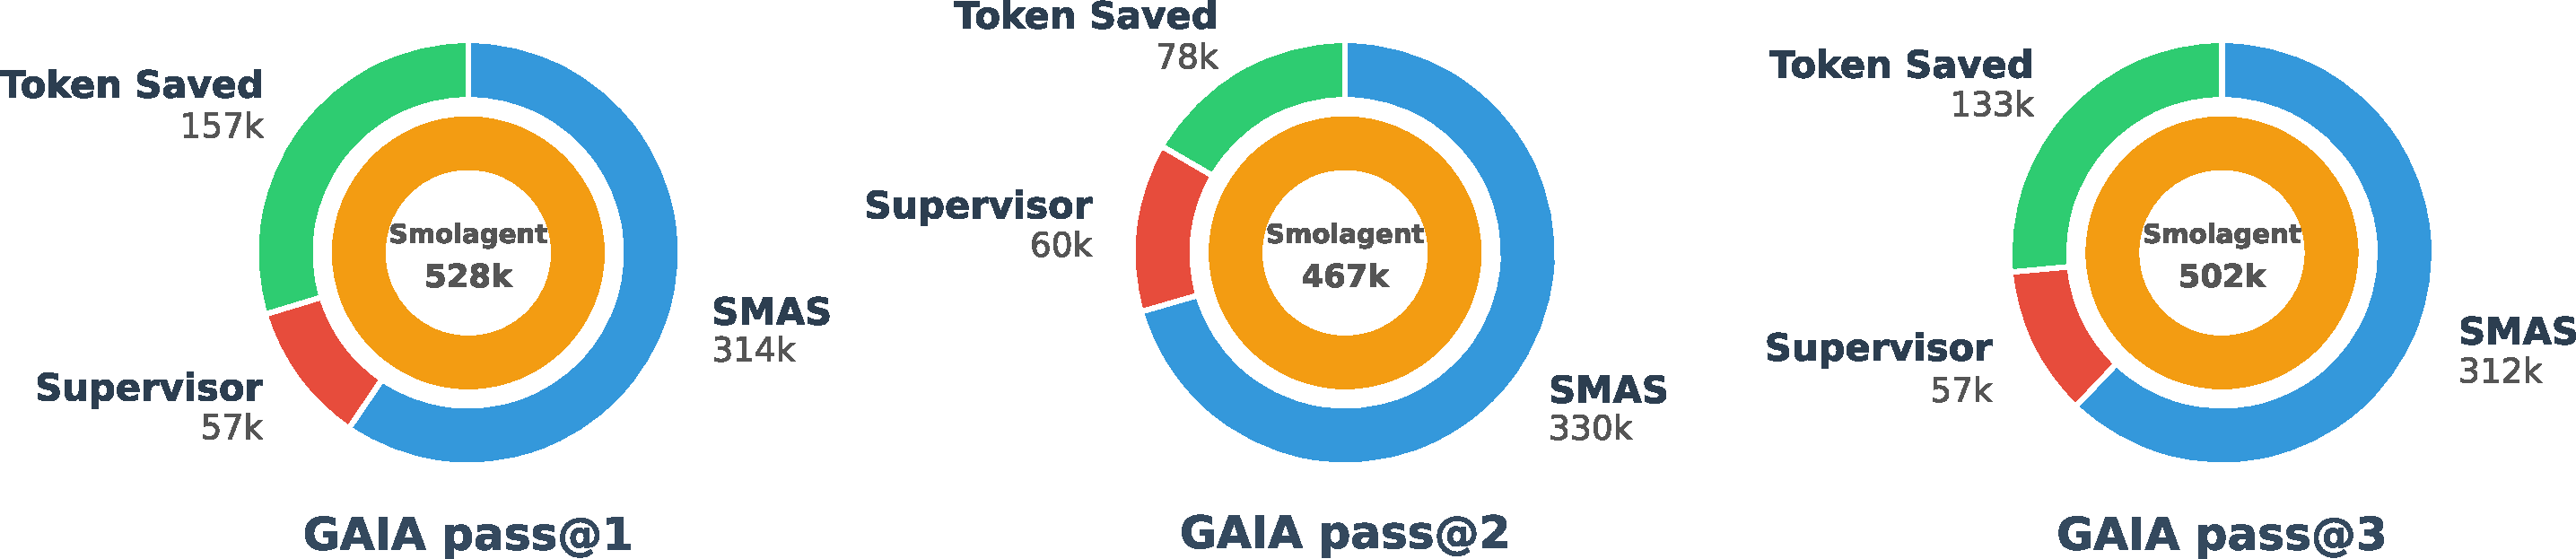
\includegraphics[width=0.9\linewidth]{resources/figures/super_overhead.pdf}
    \vspace{-0.5em}
    \caption{
        \textbf{\method overhead on the GAIA benchmark.}
    }
    \label{fig:super_overhead}
\end{figure}


\paragraph{Latency Overhead Analysis.}
Table \ref{tab:ablation_latency} and Figure \ref{fig:super_latency} analyzes the temporal impact of \method. While integrating the supervisor introduces an average latency increase of \textbf{37.27\%}, this translates to an absolute delay of less than \textbf{1.5 minutes} per task. Crucially, the ablation study reveals that Adaptive Observation Purification is the primary driver of this latency. Notably, the \textit{w/o Purification} variant exhibits a runtime nearly identical to the baseline (236.21s vs. 233.96s). This indicates that the overhead is strictly tied to the processing of excessive information. We consider this a strategic trade-off: exchanging a modest temporal cost for substantial economic (token) savings and enhanced system robustness.

\begin{table}[!t]
    \caption{
        \textbf{Ablation study of \method's components regarding Latency} on the GAIA validation set.
        Average latency (in seconds) is reported for different complexity levels.
    }
    \label{tab:ablation_latency}
    \centering
    \resizebox{\textwidth}{!}{
        \begin{tabular}{>{\raggedright\arraybackslash}m{4cm} c c c c c}
            \toprule
            \bf Method                   & \bf Avg. Acc. & \bf Avg. Latency (s)                             & \bf Level 1 Avg. Lat. (s)                        & \bf Level 2 Avg. Lat. (s)                        & \bf Level 3 Avg. Lat. (s)                        \\
            \midrule
            Smolagent                    & 50.91         & 233.96                                           & 155.83                                           & 247.47                                           & 348.58                                           \\
            \, + SMAS (w/o Correction)   & 47.88         & 280.77 {\scriptsize \textcolor{red}{↑20.01\%}}   & 193.98 {\scriptsize \textcolor{red}{↑24.48\%}}   & 276.50 {\scriptsize \textcolor{red}{↑11.73\%}}   & 471.81 {\scriptsize \textcolor{red}{↑35.35\%}}   \\
            \, + SMAS (w/o Guidance)     & 48.48         & 271.95 {\scriptsize \textcolor{red}{↑16.24\%}}   & 211.04 {\scriptsize \textcolor{red}{↑35.43\%}}   & 291.22 {\scriptsize \textcolor{red}{↑17.68\%}}   & 332.38 {\scriptsize \textcolor{blue}{↓4.65\%}}   \\
            \, + SMAS (w/o Purification) & 49.70         & 236.21 {\scriptsize \textcolor{red}{↑0.96\%}}    & 137.00 {\scriptsize \textcolor{blue}{↓12.08\%}}  & 252.01 {\scriptsize \textcolor{red}{↑1.83\%}}    & 386.19 {\scriptsize \textcolor{red}{↑10.79\%}}   \\
            \, + SMAS                    & 50.91         & 321.15 {\scriptsize \textcolor{red}{↑37.27\%}}   & 233.11 {\scriptsize \textcolor{red}{↑49.59\%}}   & 320.93 {\scriptsize \textcolor{red}{↑29.68\%}}   & 501.31 {\scriptsize \textcolor{red}{↑43.81\%}}   \\
            \bottomrule
        \end{tabular}
    }
\end{table}

\begin{figure}[!t] %
    \centering
    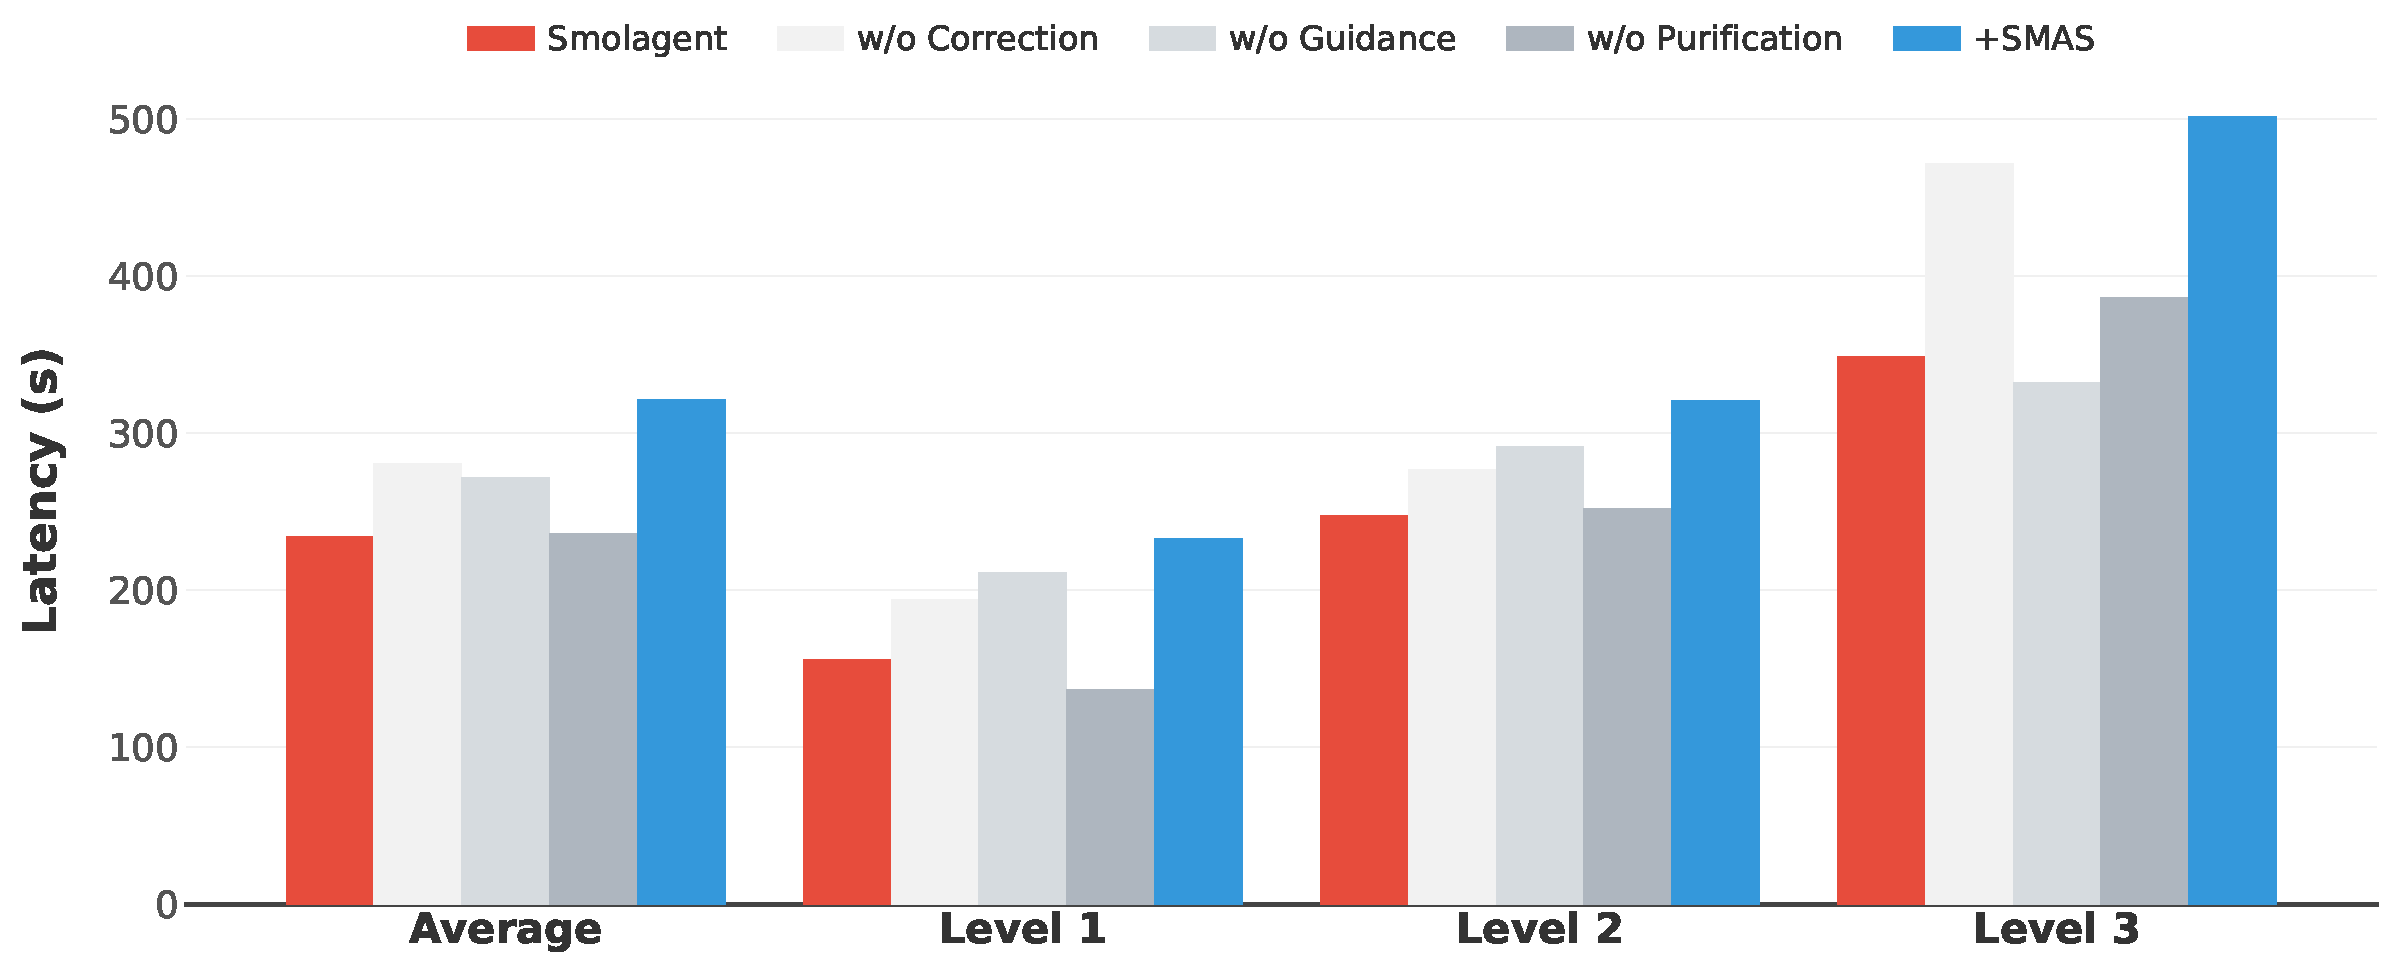
\includegraphics[width=0.9\linewidth]{resources/figures/latency_compare.pdf}
    \vspace{-0.5em}
    \caption{
        \textbf{\method latency on the GAIA benchmark.}
    }
    \label{fig:super_latency}
\end{figure}


\subsubsection{Performance Analysis on Token-Intensive Scenarios}
\label{ablation_study_subset}

Complementing the comprehensive ablation study on the full GAIA benchmark (Table \ref{tab:ablation_full}), this section zooms in on the most demanding scenarios: the top-10 most token-intensive tasks per GAIA level. This analysis aims to evaluate the scalability and robustness of \method{} under extreme computational loads.

\paragraph{Amplified Efficiency and Robustness.}
As detailed in Table \ref{tab:ablation_subset}, the benefits of \method are significantly amplified in high-complexity regimes. While the average token reduction on the full dataset is 29.68\%, SMAS achieves a remarkable \textbf{50.13\%} reduction on this intensive subset. More importantly, unlike the full dataset where accuracy remains stable, SMAS yields a distinct accuracy improvement of \textbf{6.67\%} (from 40.00\% to 46.67\%) on these hard tasks. This suggests that as task complexity and context length increase, the Supervisor's interventions become indispensable not just for cost-saving, but for enabling the agent to complete tasks that were previously intractable due to context overflow or reasoning derailment.

\paragraph{Component Contribution in Extremes.}
The ablation results on this subset reinforce the synergistic roles of our three strategies. The \textit{w/o Purification} variant shows a drastic drop in efficiency (savings drop from 50.13\% to roughly 40\%), confirming that \textbf{Adaptive Observation Purification} is the primary countermeasure against the exponential token growth in complex tasks. Meanwhile, the removal of Correction or Guidance leads to a sharp decline in accuracy back to the baseline level (40.00\%), verifying that these modules are the key safety guardrails that allow the system to navigate long-horizon tasks successfully.



\begin{table}[!t]
    \caption{
        \textbf{Ablation study of \method's components} on the subset of GAIA benchmark (top-10 most token-intensive tasks per GAIA level).
    }
    \label{tab:ablation_subset}
    \centering
    \resizebox{\textwidth}{!}{
        \begin{tabular}{>{\raggedright\arraybackslash}m{4cm} c c c c c}
            \toprule
            \bf Method                   & \bf Avg. Acc.                                & \bf Avg. Token                                   & \bf Level 1 Avg. Token                           & \bf Level 2 Avg. Token                           & \bf Level 3 Avg. Token                           \\
            \midrule
            Smolagent                    & 40.00                                        & 1,446,526                                        & 933,013                                          & 2,037,437                                        & 1,369,131                                        \\
            \, + SMAS (w/o Correction)   & 40.00                                        & 719,075 {\scriptsize \textcolor{blue}{↓50.28\%}} & 426,786 {\scriptsize \textcolor{blue}{↓54.26\%}} & 755,543 {\scriptsize \textcolor{blue}{↓62.91\%}} & 974,895 {\scriptsize \textcolor{blue}{↓28.79\%}} \\
            \, + SMAS (w/o Guidance)     & 40.00                                        & 706,831 {\scriptsize \textcolor{blue}{↓51.14\%}} & 453,623 {\scriptsize \textcolor{blue}{↓51.38\%}} & 913,109 {\scriptsize \textcolor{blue}{↓55.18\%}} & 753,761 {\scriptsize \textcolor{blue}{↓44.95\%}} \\
            \, + SMAS (w/o Purification) & 46.67{\scriptsize \textcolor{red}{↑6.67\%}}  & 851,747 {\scriptsize \textcolor{blue}{↓41.11\%}} & 585,411 {\scriptsize \textcolor{blue}{↓37.26\%}} & 990,769 {\scriptsize \textcolor{blue}{↓51.37\%}} & 979,061 {\scriptsize \textcolor{blue}{↓28.49\%}} \\
            \, + SMAS                    & 46.67 {\scriptsize \textcolor{red}{↑6.67\%}} & 721,332 {\scriptsize \textcolor{blue}{↓50.13\%}} & 522,364 {\scriptsize \textcolor{blue}{↓44.01\%}} & 960,694 {\scriptsize \textcolor{blue}{↓52.85\%}} & 680,939 {\scriptsize \textcolor{blue}{↓50.26\%}} \\
            \bottomrule
        \end{tabular}
    }
\end{table}



\subsection{Failure Mode Analysis}

While \method demonstrated robustness across benchmarks, it relies on backbone LLMs and is thus subject to their inherent limitations. We identify three primary failure modes and their implications.

\paragraph{Information Loss during Purification.} The \textit{Adaptive Observation Purification} module faces a trade-off between context reduction and information preservation. In extreme cases observed in the OAgents framework, where single observations exceeded 200,000 characters, the Supervisor risks hallucinating or omitting critical details during compression. However, our empirical results suggest that the system's resilience to context overflow generally outweighs the cost of granular information loss, as evidenced by the overall token savings and success rates (see in Table \ref{tab:mas-agnostic}).

\paragraph{Ineffective Guidance and Loops.} The \textit{Inefficiency Guidance} module may occasionally provide suboptimal advice or fail to break a stubborn loop. To mitigate the risk of the Supervisor itself becoming a source of latency (e.g., engaging in an infinite correction loop with a non-responsive agent), we enforce a hard constraints of maximum \textit{two} guidance interventions per sub-task. While this design prioritizes bounded latency over guaranteed resolution for the hardest tasks, it effectively prevents runaway costs.

\paragraph{Variance in Trigger Frequency across Backbones.} Contrary to the assumption that a supervisor acts uniformly, our analysis reveals that \method exhibits different operational behaviors depending on the backbone model's capability. For instance, as shown in our logs with Qwen3-235B, less capable models trigger the \textit{Error Correction} module significantly more often due to frequent basic failures (e.g., malformed JSON tool calls). This frequent firing increases the Supervisor's token overhead, partially explaining the lower net token savings compared to GPT-4.1 (see in Figure \ref{fig:model-agnostic}). Conversely, stronger models may trigger supervision too rarely if the heuristic filter is not sensitive enough to their subtle logic errors. This highlights that while the \textit{framework} is model-agnostic, the \textit{efficiency gains} are correlated with the backbone LLM's adherence to instruction following.

\subsection{Case Study}
\label{case_study}

\begin{mdframed}[backgroundcolor=white!10,linecolor=black,linewidth=2pt,roundcorner=8pt]
    \textbf{\color{black!80}GAIA Benchmark Case Information}
    \vspace{5pt}
    \hrule
    \vspace{8pt}
    \textbf{Task ID}: 5b2a14e8-6e59-479c-80e3-4696e8980152 \\ \\
    \textbf{Level}: 3 \\ \\
    \textbf{Question}: The brand that makes these harnesses the dogs are wearing in the attached pic shares stories from their ambassadors on their website. What meat is mentioned in the story added Dec 8th 2022? \\ \\
    \textbf{Attached iamge}: 5b2a14e8-6e59-479c-80e3-4696e8980152.jpg
\end{mdframed}

\begin{tcolorbox}[
        colback=gray!5!white,
        colframe=gray!50!black,
        title=Smolagent,
        floatplacement=Hp,
        breakable  %
    ]
    \textbf{1. Activate first search\_agent}:\\
    \textbf{Failure attribution}: page\_down 10 times and end up searching \\
    \textbf{Output of first search\_agent}:
    \begin{lstlisting}[basicstyle=\ttfamily\small, breaklines=true, columns=fixed, breakindent=0pt, xleftmargin=0pt, gobble=0]
Observations: ### 1. Task outcome (short version):
Despite a detailed investigation and navigation through the RC Pets official website and blog section, I was unable to locate the ambassador story posted on December 8th, 2022. Therefore, I cannot report any mention of meat in its content.
\end{lstlisting}
    \textbf{2. Activate another search\_agent}:
    \begin{itemize}[leftmargin=1em]
        \item Plan: turn to access historical versions of the website
        \item page\_down for 7 times
        \item Then web\_search other resources
        \item Output of search\_agent
              \begin{lstlisting}[basicstyle=\ttfamily\small, breaklines=true, columns=fixed, breakindent=0pt, xleftmargin=0pt, gobble=0]
Observations: ### 1. Task outcome (short version):
Despite a detailed investigation and navigation through the RC Pets official website and blog section, I was unable to locate the ambassador story posted on December 8th,2022. Therefore, I cannot report any mention of meat in its content.
\end{lstlisting}
    \end{itemize}
    \textbf{3. Activate third search\_agent}:
    \begin{itemize}[leftmargin=1em]
        \item Plan: Thought: Since all direct website and archive attempts failed, I will extend my search to include RC Pets' official social media (Instagram, Facebook, Twitter) and broader web, as brands often share ambassador stories across platforms and tag or date posts.
        \item web\_search for 8 times
        \item Output of search\_agent
              \begin{lstlisting}[basicstyle=\ttfamily\small, breaklines=true, columns=fixed, breakindent=0pt, xleftmargin=0pt, gobble=0]
Observations: ### 1. Task outcome (short version):
No evidence was found of any RC Pets ambassador or partner story posted on December 8th, 2022, on official RC Pets Instagram, Facebook, Twitter, or the broader web. No blog posts, community group stories, or ambassador reposts regarding RC Pets for that date or month could be 
located, and no relevant content mentioning meat was found.
\end{lstlisting}
    \end{itemize}
    \textbf{Original final answer}:
    \begin{lstlisting}[basicstyle=\ttfamily\small, breaklines=true, columns=fixed, breakindent=0pt, xleftmargin=0pt, gobble=0]
Final answer: After an exhaustive investigation across all available RC Pets channels (official website, blog, and social media), Wayback Machine, pet influencer blogs, hashtags, and pet community forums, no ambassador story or repost by RC Pets or affiliated 
ambassadors/partners could be found for December 8th, 2022. No story mentioning any meat was identified for the date or month, and no content relevant to the request is accessible through any official or community web source. All logical avenues for retrieving the answer were 
attempted and exhausted.
\end{lstlisting}
    \textbf{Reformulated answer}: Unable to determine
\end{tcolorbox}


\begin{tcolorbox}[
        colback=gray!5!white,
        colframe=gray!50!black,
        title=Smolagent + SupervisorAgent,
        floatplacement=Hp,
        breakable  %
    ]
    \textbf{Supervision type: Basic\_extraction} - 8 times\\
    \textbf{Supervision type: Inefficiency\_analysis} - 2 times
    \begin{itemize}[leftmargin=1em]
        \item First time
              \begin{lstlisting}[basicstyle=\ttfamily\small, breaklines=true, columns=fixed, breakindent=0pt, xleftmargin=0pt, gobble=0]
guidance: Providing guidance to agent: 'Stop paging through the blog manually. Instead, use the web\_search tool or the Ruffwear website's internal search to find the specific ambassador story posted on December 8th, 2022. You could search for 'Ruffwear ambassador story December 8 2022' or check if the blog section has a date-filter or text search. Once you locate the precise article, examine it for any mention of meat, noting a quote for context.'
\end{lstlisting}
              \begin{lstlisting}[basicstyle=\ttfamily\small, breaklines=true, columns=fixed, breakindent=0pt, xleftmargin=0pt, gobble=0]
Analysis: The agent is stuck repeatedly using 'page\_down' without making meaningful progress toward locating the December 8th, 2022 story among the 'ambassadors' blog entries. There are 82 pages, and there's no indication the agent is close to the correct blog post. This paginated browsing is highly inefficient when a direct search or filter by date would be much faster. It's overwhelmingly more efficient to instead search for the specific blog post by date ('December 8th, 2022') using the web\_search tool or any site search functionality if available.
\end{lstlisting}
        \item Second time
              \begin{lstlisting}[basicstyle=\ttfamily\small, breaklines=true, columns=fixed, breakindent=0pt, xleftmargin=0pt, gobble=0]
approve
\end{lstlisting}
    \end{itemize}

    \textbf{Supervision type: sub\_agent\_result\_synthesis} - 1 time
    \begin{itemize}[leftmargin=1em]
        \item Original output length: 47902
        \item Length after process: 1438
              \begin{lstlisting}[basicstyle=\ttfamily\small, breaklines=true, columns=fixed, breakindent=0pt, xleftmargin=0pt, gobble=0]
content = """
### Official Ruffwear Ambassador Stories Section
- Ruffwear ambassador stories are shared in 'Explored: A Ruffwear Blog' (https://ruffwear.com/blogs/explored/tagged/ambassadors).

### Story Posted December 8, 2022
- Title: "Snow Camping With Theresa & Cassie"
- Author: Theresa Silveyra
- Date Published: December 8, 2022 ("2022-12-08 08:00:01 -0800")
- Story URL: https://ruffwear.com/blogs/explored/snow-camping-with-theresa-cassie

### Meat Mentioned in the Story
- The only specific meat mentioned is "bacon".

> Specific quoted context from the story:
> "Of course, barely a minute had passed before Cassie's longing eyes and dangling tongue signaled a desire to play or, perhaps, a desire for treats. She led the way back, her fluffy white tail raised high in excitement, ready to take on this new year and, more likely, ready to devour the New Year's Day bacon being cooked up in camp."

### Confirmation of Accuracy
- The article and details are confirmed by both page metadata and direct content search.
- Searches for "meat", "chicken", "beef", "turkey", "pork", "fish", "salami", and "sausage" yielded no other results; only bacon was present.

### Additional Context
- Author attribution and publication date are validated.
- Other foods or treats are referenced, but bacon is the only explicit meat in the text.

### Direct Answer
- The meat mentioned in the Ruffwear ambassador story posted on December 8th, 2022 is bacon.
"""
\end{lstlisting}
    \end{itemize}
\end{tcolorbox}


\subsection{Prompts}
\label{appendix:prompt}
\begin{tcolorbox}[
        colback=gray!5!white,
        colframe=gray!50!black,
        title=\textbf{Base prompt} for \method,
        floatplacement=Hp,
        breakable  %
    ]
    \begin{lstlisting}[basicstyle=\ttfamily\small, breaklines=true, columns=fixed, breakindent=0pt, xleftmargin=0pt, gobble=0]
base_prompt = f"""
Role: You are an expert supervisor in a multi-agent system. Your role is to monitor an agent's actions, ensure alignment with the main goal, correct errors, and optimize the workflow.

Objective: The overall objective (Global Task) is: "{global_task}"

Agent context:
You are currently reviewing an action from the agent '{agent_name}'.
This agent's specific sub-task (Local Task) is: '{local_task}'.
Here is the current local execution trace: {local_trace_str}
Here is the summary of the agent's latest thought process and the resulting observation:
    {summary}
    {current_state_summary}
    
Rules:
1.  Assess Necessity: First, assess if intervention is truly necessary. If the agent's action and observation are correct and productive, use the "approve" action. Avoid unnecessary interventions.
2.  Be Decisive: When an intervention is needed, choose the most effective action to move the project forward.
3.  Output Format: Your response MUST be a valid JSON object.

Actions:
Your available actions are: 
-  `approve`: The agent's action is correct and requires no changes. 
-  `correct_observation`: The observation contains errors or can be significantly improved (e.g., filtered, summarized, extracted). You will provide a corrected version. 
-  `provide_guidance`: The observation is correct, but the agent's thinking or next step is flawed. You will provide a hint or corrected reasoning to guide the agent. 
-  `run_verification`: You have doubts about the factual accuracy of the observation and need an external assistant to verify it. 

Your response MUST be a JSON object with the following structure:
{
  "analysis": "Your brief analysis of the situation, explaining your reasoning for the chosen action.",
  "action": "ONE of the available actions: ['approve', 'correct_observation', 'provide_guidance', 'run_verification']",
  "parameters": {
      "new_observation": "IF action is 'correct_observation', provide the refined observation here.",
      "guidance": "IF action is 'provide_guidance', provide a clear hint or instruction for the agent's next thought process.",
      "task": "IF action is 'run_verification', provide the verification question for the assistant."
  }
}"""

\end{lstlisting}
\end{tcolorbox}

\begin{tcolorbox}[
        colback=gray!5!white,
        colframe=gray!50!black,
        title=Prompt for "error\_occurrence",
        floatplacement=Hp,
        breakable  %
    ]
    \textbf{Base Prompt:}
    \begin{lstlisting}[basicstyle=\ttfamily\small, breaklines=true, columns=fixed, breakindent=0pt, xleftmargin=0pt, gobble=0]
...
\end{lstlisting}
    \textbf{Addtional Prompt:}
    \begin{lstlisting}[basicstyle=\ttfamily\small, breaklines=true, columns=fixed, breakindent=0pt, xleftmargin=0pt, gobble=0]
f"""
**Role**:You are an expert Debugger and AI Diagnostician. Your primary goal is to understand the root cause of an error and provide the most effective solution to get the agent back on track.

**Situation**:
The agent's last action resulted in a critical error, which is detailed in the "summary" of the agent's action below. **Approval is not an option; you must intervene.**

**--- Your Debugging Framework (MANDATORY) ---**
Before generating your JSON output, you MUST follow this structured thinking process:

**Step 1: Analyze the Error**
    - What is the precise error message and type (e.g., `Tool Error`, `Python Exception`, `APIError`)?

**Step 2: Examine the Context**
    - Review the `local_execution_trace` and the agent's `thought` process leading to the error.
    - What was the agent *trying* to accomplish?
    - Was the tool call or code it executed (`summary` section) syntactically correct but logically flawed?

 **Step 3: Root Cause Diagnosis**
    - Based on the error and context, what is the single most likely root cause?
    - (e.g., "The agent passed a natural language string to a tool expecting a mathematical expression.", "The agent is trying to access a file that does not exist.")

**Step 4: Formulate a Solution Strategy**
    - Based on the root cause, determine the best intervention:
        - If the error can be fixed by correcting the agent's **next thought process or action**, choose `provide_guidance`. This is the most common case for logical errors.
        - If the error was caused by faulty information in the **previous observation** that the agent is now acting upon, choose `correct_observation`.
        - If you lack critical information to solve the error and need to consult an external source, choose `run_verification`.

**--- YOUR ACTIONABLE OUTPUT (JSON) ---**
Based on your diagnosis, provide your final decision in the JSON format.
\end{lstlisting}
\end{tcolorbox}



\begin{tcolorbox}[
        colback=gray!5!white,
        colframe=gray!50!black,
        title=Prompt for "inefficiency\_behavior",
        floatplacement=Hp,
        breakable  %
    ]
    \textbf{Base Prompt:}
    \begin{lstlisting}[basicstyle=\ttfamily\small, breaklines=true, columns=fullflexible,xleftmargin=0pt]
...
\end{lstlisting}
    \textbf{Additional Prompt:}
    \begin{lstlisting}[basicstyle=\ttfamily\small, breaklines=true, columns=fixed, breakindent=0pt, xleftmargin=0pt, gobble=0]
f"""
**Role**:You are a pragmatic and experienced AI workflow strategist. Your primary goal is to ensure the agent team achieves its task in the most efficient way **from its current state**.

**Situation**:An inefficiency trigger has been activated for agent '{agent_name}'. **This is a flag for you to review, NOT a confirmation of a problem.** The agent might be engaged in a necessary, methodical process.

**Global Execution Trace**:
{global_trace_str}

**--- Your Decision Framework (MANDATORY) ---**
Before generating your JSON output, you MUST follow this structured thinking process:

**Step 1: Goal & Plan Inference**
    - Based on the `Global Execution Trace`, what is the agent's immediate, implicit plan?
    - (e.g., "The agent is clearly trying to collect all rows of a data table by repeatedly using `page_down`.")

**Step 2: Progress Assessment**
    - Is the agent making tangible progress towards its inferred goal?
    - Is each new step yielding new, relevant information (even if it's just more rows of the same table)?
    - How close is the agent to completing this sub-task? (e.g., "It is on page 10 of 13, it is very close to getting all the data.")

**Step 3: Cost-Benefit Analysis of Intervention**
    - **Compare two costs**:
        - **Cost A**: The estimated cost (time, tokens) of letting the agent **continue** its current, perhaps clumsy, path to completion.
        - **Cost B**: The estimated cost of **interrupting** the agent, guiding it to a new path, and having it **start over** on that new path.
        - **CRITICAL QUESTION**: Is the agent "one step away" from solving its sub-task? If so, interrupting it is almost always the wrong decision, even if a theoretically "better" path exists.

**Step 4: Decision and Justification**
    - Based on the analysis above, decide between `approve` and `provide_guidance`.
    
**--- YOUR ACTIONABLE OUTPUT (JSON) ---**
You must choose ONE of the following two actions:

**1. If you decide the agent should continue:**
    - **Condition**: The agent is making clear, incremental progress AND is close to completing its sub-task (Cost A < Cost B).
    - **Action**: MUST be `"approve"`.
    - **Analysis**: Briefly explain *why* the agent's current path, while perhaps repetitive, is the most pragmatic way forward from its current state. (e.g., "The agent is methodically paginating through a table to gather all data. Although repetitive, this is a valid and necessary process. It is on page 10 of 13 and about to succeed. Intervention would be disruptive.")

**2. If you decide the agent is truly stuck:**
    - **Condition**: The agent is in a non-productive loop (e.g., getting the same observation repeatedly) OR the alternative path is overwhelmingly more efficient and the agent is not close to finishing (Cost B << Cost A).
    - **Action**: MUST be `"provide_guidance"`.
    - **Analysis**: Briefly explain the root cause of the inefficiency.
    - **Guidance**: The `guidance` parameter MUST contain a clear, concrete, and actionable instruction that represents a *significantly* better strategy. (e.g., "Instead of scrolling, use the `web_search` tool with the query 'who had the most BB for the 1977 Yankees' to get the answer directly.")
"""
\end{lstlisting}
\end{tcolorbox}

\begin{tcolorbox}[
        colback=gray!5!white,
        colframe=gray!50!black,
        title=Prompt for "excessive observation length",
        floatplacement=Hp,
        breakable  %
    ]
    \begin{lstlisting}[basicstyle=\ttfamily\small, breaklines=true, columns=fixed, breakindent=0pt, xleftmargin=0pt, gobble=0]
f"""
# Role: AI Agent Observation Compressor
You are a specialized data compression model for an AI agent. Your sole purpose is to process raw observations (HTML, text, etc.) and reduce their token count while strictly preserving their structural integrity and all potentially useful information.

**## Core Principles ##**
1.  **Context-Agnostic:** You have NO knowledge of the agent's overall goal or past actions. Do NOT try to infer the task. Your compression must be generic and unbiased, preserving information that could be useful for ANY potential task.
2.  **Preservation Over Compression:** It is critically important to avoid over-summarization. Losing a potentially key piece of information is a greater failure than not compressing enough. The output must retain enough detail for the agent to make informed decisions.
3.  **Structural Integrity:** The output's structure (headings, lists, paragraphs, HTML hierarchy) must mirror the input's structure. Do not merge distinct sections.
4.  **Preserve Metadata**: Always keep leading lines like `"Address: ..."`, `"Viewport: ..."` verbatim. 

**##Compression Rules##**
Based on the type of content, apply the following rules:
    
### **Type 1: For HTML Content**
    Your goal is to simplify the HTML to its semantic and structural core, removing presentation-focused noise.
    1.  **Simplify Tags:** Remove non-essential attributes.
        -   **REMOVE attributes like:** `class`, `id`, `style`, `onclick`, `onmouseover`, and any `data-*` or `js-*` attributes. These are primarily for styling and scripting, not for content structure.
        -   **KEEP essential attributes:** `href`, `src`, `alt`, `title`, `aria-label`, `placeholder`, `value`. These attributes contain crucial information for navigation and interaction.
    2.  **Remove Non-Visible Content:** Completely remove `<script>`, `<style>`, and HTML comment `` blocks.
    3.  **Preserve Content:** Keep ALL text content within tags exactly as it is. Do not summarize the text inside the HTML.
    4.  **Whitespace:** Condense multiple spaces, newlines, and tabs in the HTML structure into a single space where appropriate to improve readability without losing structure.
    **Example:**
        * **Original:** `<td class='datacolBoxR' style='padding: 5px;'><a href="/wiki/some_link" title="Some Link">25</a></td>`
        * **Compressed:** `<td><a href="/wiki/some_link" title="Some Link">25</a></td>`

### **Type 2: For Plain Text Content**
    Your goal is to make the text more concise without losing factual information or its original layout.
    1.  **Retain Key Information:** Fully preserve all named entities (e.g., people, organizations, locations), numbers, dates, codes, IDs, and any factual data.
    2.  **Condense Prose:** For descriptive sentences or paragraphs, rephrase them to be more direct. Remove filler words, redundant phrases, and overly elaborate adjectives. However, do NOT eliminate the sentence entirely.
    3.  **Maintain Structure:** If the input text has multiple paragraphs, bullet points, or numbered lists, the output MUST have the same structure. Do not flatten a list into a single paragraph.
    **Example:**
        * **Original:** "The company, officially known as The International Business Machines Corporation (IBM), is a very large and influential American multinational technology corporation that has its headquarters located in Armonk, New York, and it was originally founded all the way back in 1911."
        * **Compressed:** "The International Business Machines Corporation (IBM) is an American multinational technology corporation headquartered in Armonk, New York, founded in 1911."

**## Final Instruction ##**
Process the following observation according to the rules above. Provide only the compressed output, without any extra text, explanation, or preamble.
    {observation}
"""
\end{lstlisting}
\end{tcolorbox}


\begin{tcolorbox}[
        colback=gray!5!white,
        colframe=gray!50!black,
        title=Prompt for "result\_synthesis",
        floatplacement=Hp,
        breakable  %
    ]
    \# this is for synthesis the final answer from sub-agent

    \textbf{Base Prompt:}
    \begin{lstlisting}[basicstyle=\ttfamily\small, breaklines=true, columns=fixed, breakindent=0pt, xleftmargin=0pt, gobble=0]
  ...
  \end{lstlisting}
    \textbf{Additional Prompt:}
    \begin{lstlisting}[basicstyle=\ttfamily\small, breaklines=true, columns=fixed, breakindent=0pt, xleftmargin=0pt, gobble=0]
  f"""
  **Role**:You are an expert Intelligence Analyst working for a manager agent. Your task is to process a verbose report from a sub-agent (e.g., a search specialist) and synthesize a direct, comprehensive, and clean answer for your manager.
  
  **--- YOUR INPUTS ---**
  **1. The Manager's Request (Immediate Goal)**:
      - "{local_task}"
  
  **2. The Overall Mission (Global Goal)**:
      - "{global_task}"
  
  **3. The Sub-Agent's Full Field Report (Raw Observation)**:
       ```
      {summary} 
      ```
  (Note: The 'summary' variable here contains the sub-agent's full, multi-part final_answer)
  
  **--- YOUR CRITICAL TASK ---**
  Your sole task is to read the ENTIRE "Field Report" (including the short version, detailed version, and the summary of work) and synthesize a single, clean, and self-contained response that **fully and completely** answers the "Manager's Request".
      **Critical Rule for Synthesis**:
      **Preserve Semantic Structure**: When synthesizing, you MUST maintain the original information's hierarchy. If the source contains headings, chapters, articles, or numbered/bulleted lists, these structural elements **MUST be preserved** in your output to give context to the data points below them. **Do not flatten a structured document into a simple, unstructured block of text.**
      **Your Internal Thought Process (MANDATORY)**:
          1.  **Deconstruct the Manager's Request**: What are the specific pieces of information the manager is asking for? Create a mental checklist.
          2.  **Scan the Entire Report**: Read all parts of the sub-agent's report to find the answers for your checklist. The most valuable details are often in the "extremely detailed version" or the "summary of work".
          3.  **Synthesize, Don't Just Extract**: Combine the findings into a coherent, fluent, and direct answer. Do not simply copy the "short version". Your answer must be comprehensive enough to prevent the manager from needing to ask follow-up questions.
          
  **Example**:
  - **Manager's Request**: "Find the number of encoder layers in the BERT-Base model."
  - **Sub-Agent's Report**: (A long text containing "Short version: 12 layers", "Detailed version: ...Section 3 of the paper states L=12 for BERT-Base...", etc.)
  - **Your Ideal Synthesized Output**: "The BERT-Base model has 12 encoder layers (L=12), as specified in Section 3 of the original paper by Devlin et al., 2018."
  
  **Action**:Your action MUST be `"correct_observation"`.
  
  **Parameter**:Provide your final, synthesized answer in the `"new_observation"` parameter.
  """
  \end{lstlisting}
\end{tcolorbox}
